\documentclass[a4paper, fontsize=11pt, abstract=on, listof=totoc, bibliography=totoc, twoside=false]{scrreprt}
\usepackage{scrlayer-scrpage}
\usepackage{mathtools}
\usepackage{fontspec}
\defaultfontfeatures{Ligatures=TeX, Scale=MatchLowercase}
\newcommand{\euro}{€}
\usepackage[usenames, dvipsnames]{xcolor}
\usepackage{polyglossia}
\setdefaultlanguage[spelling=new]{german}
\setotherlanguage[variant=british]{english}
\usepackage[autostyle=true]{csquotes}
\renewcommand{\mkblockquote}[4]{\openautoquote#1\closeautoquote#2#4#3}
\usepackage[backend=biber, style=iso-authoryear]{biblatex}
\addbibresource{bib/main.bib}
\usepackage[section]{placeins}
\usepackage{scrhack}
\usepackage{listings}
\usepackage{longtable, booktabs}
\usepackage{graphicx, grffile}
\usepackage[unicode=true]{hyperref}
\usepackage[acronym, toc]{glossaries}
\newacronym{AJAX}{AJAX}{Asyncronious JavaScript And XML}
\newacronym{API}{API}{Application Programming Interface}
\newacronym{JSON}{JSON}{JavaScript Object Notation}
\newacronym{ORM}{ORM}{Objekt-Relationalen-Mapper}
\newacronym{RAM}{RAM}{Random-Access-Memory}
\newglossaryentry{ACID}{name={Atomicity, Consistency, Integrity and Durability},
description={ACID steht für Atomarität, Konsistenz, Integrität und
Widerstandsfähigkeit. Alle diese Begriffe stehen im Zusammenhang mit Konsistenz
der Daten einer relationalen Datenbank. Bei ACID muss nach einer Transaktion auf
allen Knoten der selbe Zustand sein.}}
\newglossaryentry{BASE}{name={Basically Available, Soft State,
Eventually Consistent}, description={BASE ist der Gegenpart zu \gls{ACID} für
NoSql-Systeme. Bei BASE geht es darum die Konsistenz der Verfügbarkeit
unterzuordnen. Im Gegensatz zu ACID muss bei BASE irgendwann der selbe Zustand
sein. Der genau Zeitpunkt ist jedoch nicht definiert.}}
\newglossaryentry{CAP}{name={Consistency, Availability, Partition Tolerance},
description={CAP steht für Konsistenz, Verfügbarkeit und Ausfalltoleranz und ist
eine Theorem von Eric Brewer. Das Theorem sagt aus, dass man lediglich zwei der
drei Eigenschaften gleichzeitig einhalten kann, die dritte wird man nie
einhalten können. \cite{Brewer2000}}}

\makeglossaries
\setlength{\parskip}{\medskipamount}
\begin{document}
\author{Mirko Lelansky}
\title{Projektbericht}
\subtitle{Vergleich von verschiedenen NoSql Schlüssel-Wert-Systemen}
\date{09.07.2017}
\maketitle
\clearpage
\begin{abstract}
\end{abstract}
\begin{english}
\begin{abstract}
\end{abstract}
\end{english}

\clearpage
\tableofcontents
\clearpage
\printglossary[type=acronym, title=Abkürzungsverzeichnis, toctitle=Abkürzungsverzeichnis]
\chapter{Einleitung}

In der heutigen Welt werden täglich große Datenmengen erzeugt. Sei es im
privaten Umwelt durch die Benutzung von Social-Media-Plattformen wie Facebook,
Twitter, \ldots oder in der Wirtschaft durch Börsendaten, medizinische
Bilddaten, \ldots . Im Zuge der zunehmenden Vernetzung von
Alltagsgegenständen wie Fernseher, Kühlschrank, \ldots, welches man auch als
IoT\footnote{Internet of the Thinks} bezeichnet, stieg die täglich erzeugte
Datenmenge nocheinmal sehr stark an.

Diese Daten können dabei strukturiert, semi-strukturiert oder unstrukturiert
sein. Strukturierte Daten können sehr leicht von Maschinen verarbeitet werden,
da sie über eine fest vorgegeben Struktur verfügen. Im Gegensatz dazu haben
semi-strukturiete Daten eine lose Struktur, dies bedeuted, dass definiert ist,
wie einzelne Bausteine auszusehen haben, jedoch nicht wie das Dokument aus den
definierten Bausteinen entsteht. Über unstrukturierte Daten kann lediglich die
Aussage treffen, um welchen Typ von Daten es sich handelt, also zum Beispiel,
ob es ein Bild ist.

Diese riesigen unterschiedliche strukturierten Daten müssen effizient
gespeichert und verarbeitet werden, damit ein Mehrwert entstehen kann.
Relationale Datenbanksysteme stoßen dabei schnell an ihre Grenzen. Für solche
Zwecke ist es besser alternative Systeme einzusetzen wie NoSql-Systeme.

\section{Motivation}

Wie schon erwähnt sind NoSql-Systeme bei semi- und unstrukturieten Daten besser
geeignet. Jedoch gibt es eine vielzahl von unterschiedlichen NoSql-Systemen,
die alle für einen gewissen Einsatz entwickelt wurden. Um deshalb eine
Entscheidung treffen zu können, welches System man einsetzen möchte, muss man
die verschiedenen Systeme vergleichen. Dabei spielen nicht nur die Funktionen
der einzelnen Systeme eine Rolle, sondern auch eventuell vorhandene
Bibliotheken.

Im weiteren Verlauf dieser Arbeit werden wir die Key-Value-Systeme als einen
Typ herausnehmen und davon mehrere Systeme und deren Integration vergleichen.

\section{Ziel der Arbeit}

Ziel der Arbeit ist es die Key-Value-Stores Redis, Memcached und ein frei
wählbares System hinsichtlich ihrer Eigenschaften zu untersuchen. Dabei soll
vor allem der Fokus auf Leistung\footnote{Performance} und verteieltes
Rechnen\footnote{Clustering} gelegt werden. Redis verfügt über ein
eigenes System „redis-benchmark“, welches ausgeführt und mit den eventuell
vorhanden Werkzeugen der anderen Systeme verglichen werden soll. Dabei kann es
notwendig werden das Werkzeug für die anderen System anzupassen.

Außerdem sollen die existierenden
Zugriffsbibliotheken\footnote{Client-Libraries} der Systeme verglichen
werden. Der Fokus soll hierbei auf der Programmiersprache Python liegen. Dazu
sollen gegeignete Anwendungsfälle ausgedacht und umgesetzt werden.

\section{Aufbau der Arbeit}


Im ersten Kapitel werden beteiligten Technologien und Softwaresysteme
beschrieben, um einen Überblick zu bekommen. Danach wird das bestehende
Benchmark-Werkzeug von Redis analysiert und der Entwurf für die anderen beiden
Key-Value-Stores beschrieben. Außerdem wird der Use-Case beschrieben, der dann
mit Hilfe der Python-Bibliotheken umgesetzt wird. Anschließend wird die
technische Umsetzung beschrieben sowohl des Bechmark-Tools als auch des
umgesetzten Use-Cases. Abschließend folgt die Zusammenfassung der Ergebnisse
und der Ausblick in die Zukunft.

\chapter{Theoretische Grundlagen}
In diesem Kapitel werden die für die Realisierung benötigten Technologien und
Methoden beschrieben.

Dazu wird zuerst erklärt, was man unter NoSql versteht und eine kurze Zeitlinie
der Entwicklung. Anschliend werden die verschiedenen Arten von NoSql und
speziell von Schlüssel-Wert-Systemen beschrieben.

Danach folgt der Vergleich von Redis, Memcached und Voldemort. Dazu werden
zuerst die jeweiligen Systeme erläutert. Anschließend folgt der eigentliche
Vergleich, dazu werden die jeweiligen Eigenschaften kurz erläutert und danach
wie die jeweiligen Systeme dies umsetzen.

\section{NoSql}
NoSql-Systeme sind keine neue Erfindung, sondern entwickelten sich quasi
parallel mit den relationalen Systemen. Der Grund warum erst jetzt NoSql einen
so großen Durchbruch erfährt, hängt vor allem mit dem BigData-Gedanken zusammen.
Vor BigData war es üblich die Geschäftsdaten auf wenigen Datenbank-Server zu
speichern. Mit der Entwicklung der Sozialen-Netzwerke und der zuhnemenden
Vernetzung von Alltagsgegenständen stieg die erzeugte Datenmenge rapide auf
Peta-, Exa-Byte Bereich an. Dies hatte zur Folge, dass sich die Geschäftdaten
mit herkörmlichen Mitteln nicht mehr effektiv Speichern und verarbeiten liesen
und man nach Alternativen gesucht hat, den NoSql-Systemen.
Obwohl der NoSql Begriff heute so eine Aktualität besitzt, gibt es keine bis
heute keine einheitliche Begriffsdefinition. Vielmehr ist NoSql ähnlich wie
AJAX ein Sammelbegriff für verschiedene Technologien und Ideen. Während früher
NoSql wörtlich für „no Sql“ also "kein Sql" stand steht es heute eher für
„not only Sql“ also "nicht nur Sql". Auch ab wann man ein System als
NoSql-System zählt, ist nicht klar geregelt. Vielmehr gibt es eine Reihe von
Punkten, die ein System erfüllen kann wie: \cite{Edlich2011}

\begin{itemize}
\item Das zugrundeliegende Datenmodell ist nicht relational.
\item Die System sind von Anbeginn auf eine verteilelte und horizontale
Skallierbarkeit ausgerichtet.
\item Das NoSql-System ist Open-Source.
\item Das System ist schemafrei oder hat nur schwache Schemarestriktionen.
\item Aufgrund der verteielten Architektur unterstützt das System einfache
Datenreplikation.
\item Das System besitz eine einfache API.
\item Dem System liegt meist auch ein anderes Konsitenzmodell zugrunde:
Eventuelly Consistenz und BASE aber nicht ACID.
\end{itemize}

. Daraus haben sich die unterschiedlichsten Systeme entwickelt.

\subsection{Entwicklungsmeilensteine}
Der Ursprung von NoSql ist die im Jahr 1979 von Ken Thompson entwickelte
Datenbank DBM\footnote{\url{http://www.gnu.org/software/gdbm/gdbm.html}}, die
bis heute noch von Linux verwendet wird. Die ersten NoSql Datenbanken, die
heute noch existieren entsanden in den 80er-Jahren, wie Lotus Note\footnote{\url{http://www-03.ibm.com/software/products/de/ibmdomino}},
BerkleyDB\footnote{\url{http://www.oracle.com/us/products/database/berkeley-db/index.html}},
GT.M\footnote{\url{https://sourceforge.net/projects/fis-gtm/https://sourceforge.net/projects/fis-gtm/}}, \ldots .
Der Begriff NoSql wurde das erste Mal 1998 von Carlo Strozzi benutzt, der eine
relationale Datenbank entwickelt hatte jedoch ohne Sql. Der richtige Durchbruch
kam allerdings erst im Jahr 2000 mit dem Web 2.0 und den daraus resultierenden
Anstieg des Datenvolumens. Dieser Datenanstieg erforderte neue Methoden zur
effizenteren Speicherung und Verarbeitung. Google war dabei der Vorreiter mit
seinem Map-/Reduce-Ansatz. Die Idee dabei ist es, eine große Datenmenge in
kleinere Pakete aufzuteilen und diese dann unabhängig voneinander zu verarbeiten.
Anschließend werden die einzelnen Zwischenergebnisse gesammelt und zu einen
Gesammtergebnis zusammengefasst. Diese Idee ließ sich sehr gut mit den Ideen
der funktionalen Programmiersprachen umsetzen, denn dort wird auf einer Kopie
der tatsächlichen Daten gearbeitet. Später zogen die anderen großen Firmen mit
eigenen Lösungen nach und heute kann man sagen, dass es den Map-/Reduce-Ansatz
nicht mehr gibt, sondern verschiedene Implementierungen, die für einen gewissen
Einsatzzweck entwickelt wurden. Die Entwicklung der mordernen NoSql-Systemen
begann im Jahr 2005 mit Systemen wie Neo4j, Redis, Cassandra, \ldots und hält
bis heute noch an.

\subsection{Arten von NoSql-Systemen}
Wie oben schon beschrieben existieren eine Vielzahl an unterschiedlichsten
NoSql-Systemen. Dies hat zur Folge, dass es nicht leicht ist das für seinen
Anwendungsfall passende System zu finden. Deshalb kam der Gedanke NoSql-Systeme
nach bestimmten Kriterien zu sortieren um eine bessere Entscheidung treffen zu
können. Schnell entwickelten sich mehrere Kriterien. Die gröbste Einteillung,
die man vorgenommen hat, war die Einteillung in Kern-NoSql-Systeme und
Soft-NoSql-Systemen. Wobei die Grenze und der Unterschied zwischen den Gruppen
nicht klar geregelt ist. Danach werden NoSql-Systeme häufig nach ihrem
zugrundeliegenden Datenmodell eingeteilt. Nachfolgend folgt eine Einteilung der
NoSql-Systeme nach dem Datenmodell mit einer Erklärung was man sich unter dem
jeweiligen Typ vorzustellen hat und einige Vertreter davon:

\begin{itemize}
\item Kern-NoSql-Systeme
\begin{description}
\item[dokumentenbasierte Systeme] Dokumentenbasierte System speichern die Daten
in Dateien, meist im JSON-Format, ab. Zu dieser Gruppe gehören Systeme wie
MongoDB oder CouchDB.
\item[Schlüssel-Wert-Systeme] Schlüssel-Wert-Systeme speichern wie der Name schon
sagt die Daten unter einem gewissen Schlüssel ab, über den dann später die Daten
wieder gelesen werden. Zu dieser Gruppe gehören Systeme wie Redis, Voldemort,
Memcached.
\item[graphbasierte Systeme] Bei graphbasierten Systemen liegen die Daten als
Graph vor. Solche Systeme ermöglichen es leicht herauszufinden, welcher Knoten
mit einem anderen Knoten in Beziehung steht. Dies wird bei Sozialennetzwerken
bezutzt um herauszufinden, wer "Freund" von jemanden ist. Zu dieser Gruppe
gehören Systeme wie Neo4j.
\item[spaltenorientierte Systeme] Spaltenorientiert System haben Ähnlichkeiten
mit relationalen Systemen, die ja auch über Spalten verfügen. Allerdings kann man
bei einem spaltenorientierten System eine Liste von Schlüssel-Wert-Paaren
abspeichern und im Extremfall kann sogar die Spalte eine Liste von
Schlüssel-Wert-Paaren sein. Zu dieser Gruppe gehören Systeme wie HBase, Cassandra.
\end{description}
\item Soft-NoSql-Systeme
\begin{description}
\item[XML-Datenbanken]
\item[Objekt-Datenbanken]
\end{description}
\end{itemize}

.

\chapter{Design}
In diesem Kapitel geht es darum die einzelnen Benchmark-Werkzeuge zu
vergleichen. Dabei werden die einzelnen Tools analysiert und die Schwachstellen
aufgezeigt. Dazu werden für die einzelnen Schwachstellen Lösungsansätze
präsentiert bezugnehmend auf den derzeitigen Stand der Entwicklung der
jeweiligen Werkzeuge.

Des Weiteren wird der umzusetzende Anwendungsfall beschrieben. Dazu gehört, was
der Anwendungsfall zeigen soll mit einer detaillierten Architekturdarstellung
zur Visualisierung. Dabei werden auch erste getroffene Design-Entscheidungen
erläutert.

\section{Analysephase der Benchmark-Werkzeuge}
Wenn man eine eigene Anwendung entwickelt hat oder eine fremde Anwendung
integrieren möchte stellt sich schnell auch die Frage, ob die Anwendung auch für
die ursprünglich geplanten Bedürfnisse auch geeignet ist. Um diese Frage
beantworten zu können, braucht man erst einmal eine Vorstellung, welche
Grenzwerte, sogenannte Metriken, noch akzeptable sind. Danach kann man sich ein
Test-Setup überlegen, wie man die ausgewählten Metriken misst. Anschließend kann
man die gemessenen Werte mit den geplanten Werten vergleichen, ob die Anwendung
für den geplanten Einsatzzweck geeignet ist.


Dabei will man natürlich möglichst den Messvorgang automatisieren um ihn auch
mit unterschiedlichsten Konfigurationen wiederholen zu können und damit die
verschiedenen Einsatzszenarios zu testen.

\subsection{Stand der Entwicklung}
Redis hat für die Performance-Messung ein eigenes Werkzeug
\enquote{redis-benchmark}. Dieses Werkzeug ist komplett in C geschrieben. Im
Wesentlichen besteht das Werkzeug aus einer Event-Schleife für die Verarbeitung
und einem Schreibprozess auf dem Socket. Dabei wurden viele alt bekannte
Konzepte nochmals durch spezielle Wrapper gekapselt. Der Schreibprozess wurde
ausgelagert in eine neue Bibliothek \enquote{hiredis} und wird jetzt Schritt für
Schritt in den Werkzeugen eingesetzt. Das Werkzeug stellt für alle Methoden,
die Redis bereitstellt einen Test zur Verfügung.

Memcached hat kein eigenes Tool zur Messung der Performance. Erst mit Version
1.2 wird ein solches Tool \enquote{memaslab} existieren. Es gibt jedoch einige
externe Werkzeuge. Diese Werkzeuge bauen jedoch alle auf einer alten Version von
\enquote{redis-benchmark} auf. Das bekannteste Werkzeug ist dabei
\enquote{mc-benchmark}. Die Entwickler haben dabei mehr oder weniger alles
unnötige gelöscht und dann das Werkzeug angepasst. Jedoch benutzt keines der
Werkzeuge die existierende Bibliothek \enquote{libmemcached}, welche extra von
Memcached bereitgestellt wird und zusätzliche Konfiguration Möglichkeiten für
Memcached bietet. Des Weiteren unterstützen die Werkzeuge nicht alle Methoden,
die Memcached bereitstellt.

Voldemort hat ebenfalls wie Redis ein eigenes Performane-Werkzeug
\enquote{voldemort-performance-tool}, welches wie der Rest von Voldemort in Java
geschrieben ist. Das Werkzeug bietet für alle Methoden von Voldemort einen
Test an.

Außerdem gibt es noch eine Reihe anderer Werkzeuge, welche von den großen
Firmen wie Amazon, Google, Yahoo,~\dots{} bereitgestellt werden und teilweise
kostenpflichtig sind. Diese Werkzeuge sind dann aber auch in der Lage mehrere
Systeme abzudecken. Ein Open-Source Tool, welches mit Redis und Memcached
umgehen kann, ist
memtier\footnote{\url{https://github.com/RedisLabs/memtier_benchmark}}.

Aufgrund der wenigen Funktionalität und der nicht Benutzung von geeigneten
Bibliotheken. Soll hier das Memcached-Werkzeug \enquote{mc-benchmark}
umgeschrieben werden, um eine bessere Konfiguration zu ermöglichen und die
fehlenden Methoden zu unterstützen. Dadurch ist es außerdem möglich einen
besseren Bezug zum Benchmark-Werkzeug von Redis herzustellen.

\subsection{Analyse- und Desginprozess}
Bevor überhaupt auch nur eine Zeile Code entwickelt wird, erfolgt immer eine
Analyse- und Design-Phase. Dabei geht es darum die Anforderungen und Bedürfnisse
der Kunden zu erfahren und festzuhalten um damit später in der Design-Phase
bessere Entscheidungen treffen zu können. Dies ist notwendig, damit am Ende auch
das vom Kunden gewünschte Produkt abgeliefert wird. Da dies ein komplexer
Prozess ist, sind verschiedene Modelle und Methoden entwickelt worden, um diesen
Prozess zu begleiten.

Zum einen gibt es die schwergewichtigen Prozessmodelle wie zum Beispiel
\enquote{Wasserfall}. Auf der anderen Seite gibt es auch leichtgewichtige
Prozesse wie \enquote{Extrem Programming}. Daneben gibt es noch die Modelle,
die sich genau zwischen den beiden Seiten befinden. Allerdings muss man dabei
beachten, dass dies nur Modelle sind und keine konkreten Arbeitsweisen, sondern
jedes Modell muss an die jeweilige Umgebung angepasst werden. Die
schwergewichtigen Modelle legen dabei ihren Fokus auf Organisation und
Dokumentation und die leichtgewichtig Modelle legen ihren Fokus mehr auf der
Implementierung des Projektes. Egal für welches Modell man sich am Ende auch
entscheidet, kann man die Anforderung des Kunden nicht mit einem oder wenigen
Terminen vollständig erfassen, da meistens die Kunden zu Beginn des Projektes
selbst noch keine Vorstellung von der benötigten Funktionalität haben, sondern
diese erst entwickeln müssen. Die leichtgewichtig Modelle haben hierbei einen
Vorteil, da sie besser mit dynamischen Änderungswünschen des Kunden umgehen
können als die schwergewichtigen Modelle.

\subsection{Anforderungen des Benchmark-Werkzeugs}
Das umgeschriebene Programm \enquote{mc-benchmark} muss dieselbe Funktionalität
erfüllen, wie das Original. Ein Punkt ist dabei, dass die Tests konfigurierbar
sein müssen, um zum Beispiel die Serveradresse des Servers zu ändern, gegen den
die Tests gefahren werden. Der andere Punkt ist, dass die beiden bisherigen
Methoden \enquote{get} und \enquote{set} auch weiterhin unterstützt werden. Es
kann jedoch im Laufe der Entwicklung zu Änderungen kommen, wenn man auf
\enquote{libmemcached} statt \enquote{hiredis} benutzt wird.

Allerdings gibt es noch eine Reihe zusätzlicher Anforderungen. Dazu gehört,
dass die fehlenden Methoden vom Werkzeug mit abgedeckt werden sollen, wie
\enquote{add}, \enquote{replace}, \enquote{append}, \enquote{prepand},
\enquote{delete}, \enquote{incr/decr},~\dots{] . Diese Anforderung ist einfach
umzusetzen, da man auf die vorhandenen Tests zugreifen und diese ggf. anpassen
kann.

\section{Analysephase des Anwendungsfalls}
Die jeweiligen NoSql-Systeme sind alleine noch nicht sehr sinnvoll, sondern erst
in Zusammenarbeit mit einer Anwendung. Der Ablauf ist dabei immer gleich. Zuerst
wird eine Verbindung zum NoSql-System aufgebaut. Anschließend werden Daten
zwischen beiden Systemen übertragen. Abschließend wird die Verbindung wieder
abgebaut. Um nicht für jede neue Anwendung diesen Prozess neu implementieren zu
müssen, greift man auf Bibliotheken zu, welche diesen Prozess implementieren.

Für alle gängigen NoSql-Systeme und Programmiersprachen gibt es heutzutage eine
entsprechende Bibliothek oder auch mehrere, von denen meistens eine vom
Hersteller bevorzugt wird. Da der Anwendungsfall in der Programmiersprache
Python umgesetzt werden soll, kommen auch nur die Bibliothek für Python in
Frage. Dabei unterscheidet man zwischen Bibliotheken, welche rein in Python
umgesetzt sind und solchen die nur als Wrapper für die jeweiligen C Bibliotheken
dienen. Das NoSql-System Voldemort hat nur eine Python-Bibliothek, welche von
den Entwicklern bereitgestellt wird. Für Redis sind mehrere Bibliotheken
verfügbar, jedoch wird von den Herstellern die Bibliothek
redis-py\footnote{\url{http://www.github.com/andymccurdy/redis-py}} bevorzugt.
Bei Memcached gibt es mehrere Bibliotheken, welche frei wählbar sind.

\subsection{Beschreibung des Anwendungsfalls}
Als Anwendungsfall soll ein Abstimmungssystem entwickelt werden. Dabei geben
die Benutzer Bewertungen für die jeweiligen Sachen ab und ein Algorithmus
erstellt daraus eine neue Liste. Der Administrator kann neue Gegenstände ins
System einstellen. Sowohl der Administrator als auch die Benutzer können sich
jederzeit die neuste Liste ansehen.

\chapter{Realisierung}
Im diesem Kapitel geht es darum, die in der Design-Phase genannten Änderungen
praktisch umzusetzen. Dazu gehört, die einzelnen Schritte und die dabei
aufgetretenen Probleme zu erläutern. Dabei wird zuerst auf die
Benchmark-Werkzeuge und anschließend auf den Anwendungsfall eingegangen.

\section{Ausführung und Vergleich der Benchmark-Werkzeug}
Die einzelnen Benchmark-Werkzeuge und die NoSql-Systeme lassen sich nur schwer
miteinander Vergleichen, da die einzelnen Systeme sehr unterschiedliche
Funktionen bereitstellen und auch für unterschiedliche Einsatzzwecke entwickelt
wurden. So wird Memcached meist als reiner Datencache für komplette Webseiten
oder von Teilwebseiten benutzt. Während dessen ist Voldemort eher ein
Datenspeicher wie Amazons DynamoDB, Amazons S3 oder MongoDB. Dies zeigt sich
daran, dass es in Memcached und Redis sehr einfach ist einen bestehenden
Schlüssel mit einem neuen Wert abzuspeichern. Bei Voldemort ist dies nicht
einfach möglich, da bei Voldemort die einzelnen Services bzw. Server nicht
unabhängig sind. Wie auch schon in den theoretischen Grundlagen genannt wurde.
In der Regel werden in einem Cluster mehrere Versionen zu einem Schlüssel
vorhanden sein. Einige Server haben noch die alte Version, während andere Server
schon die aktuellste Version haben.

Auch spielen die unterschiedlichen Datenspeicher eine Rolle. Redis ist als
einziges System in der Lage Listen, Mengen direkt zu speichern und zu
manipulieren. Die anderen Systeme müssen den Umweg über Transformationen gehen.
Also zum Beispiel die zu speichernden Werte in JSON umwandeln und diesen dann
abspeichern. Deshalb haben die einzelnen Bechmark-Werkzeuge auch unterschiedliche
Test-Methoden.

Ein weiteres Problem sind die verschiedenen Einstellungsmöglichkeiten der
verschiedenen Tools. Die Werkzeuge Redis und Memcached erlauben eine Vielzahl
an Einstellungen vorzunehmen, wie Anzahl der Clients und Requests, Anzahl der
Datengröße. Dies ist bei Voldemort nicht möglich. Dort lässt sich nur die Anzahl
der Threads, welche die Clients darstellen, ändern. 

Die Ergebnisse der Benchmarktests sind für Redis in \ref{bench:Redis}, für
Memcached in \ref{bench:Memcached} und für Voldemort in \ref{bench:Voldemort}
dargestellt. Für Memcached und Redis sind dabei die selben Basiseinstellungen
genutzt worden. Bei Voldemort ist dies nicht möglich, da es eine andere
Konfiguration bestitzt, wie schon erwähnt wurde. 

\begin{minipage}{\linewidth}
\lstinputlisting[caption={Redis-Benchmark},label={bench:Redis}]{bench/redis-benchmark.txt}
\end{minipage}

\begin{minipage}{\linewidth}
\lstinputlisting[caption={Memcached-Benchmark},label={bench:Memcached}]{bench/memcached-benchmark.txt}
\end{minipage}

\begin{minipage}{\linewidth}
\lstinputlisting[caption={Voldemort-Benchmark},label={bench:Voldemort}]{bench/voldemort-benchmark.txt}
\end{minipage}

Man könnte nun als Basisfall die Set- und Get-Test für Memcached und Redis
viederholen und danach vergleichen in wieweit sich beide Systeme bei
unterschiedlichen Lasten verteilen. Ob es eine Konfiguration gibt, bei der Redis
besser abschneidet als Memcached. Eine größe Einschränkung ist noch zu tätigen,
da bei den Tests sowohl das zutestende System als auch das Testwerkzeug auf ein
und derselben Maschine liefen. Dies ist für einen realen Testversuch jedoch nicht
geeigntet. Da praktisch der gesammte Netzwerkverkehr wegfällt. Außerdem ist es
nicht möglich die Last auf größere Mengen hochzustellen, da sonst entweder
das Testtool oder das System durch das Betriebssystem beeinflusst würden. Wenn
jedoch nur kleine Datenmengen benutzt werden ist der Test praktisch sofort
abgeschlossen.

\subsection{Realisierung des Benchmark-Werkzeuges}
Das Benchmark-Werkzeug wurde als C-Anwendung realisiert. Dabei wurde für die
Kommandozeile, die Bibliothek gengetops benutzt, welche es ermöglicht über eine
DSL die benötigten Optionen zu definieren und den Rest der Bibliothek zu
überlassen. Dies sorgt für eine bessere Wartbarkeit der Anwendung. Darauf hin
werden die entsprechenden Test-Methoden gestartet. Dabei besteht ein
signifikanter Unterschied zwischen dem Original und der Neuentwicklung. Beim
Original laufen die Tests sequentiell ab, zuerst wird der set-Test ausgeführt
und anschließend wird der get-Test ausgeführt. Bei redis-Benchmark, wie auch
bei der Neuentwicklung können die Tests selektiert werden. Dies setzt jedoch
voraus, dass für einzelne Tests ein Setup durchgeführt werden muss, welches
früher der vorherige Test übernommen hatte. Alle Test-Methoden benutzen auch
nicht mehr direkt den Socket, sondern die von Memcached bereitgestellte
Bibliothek.

\section{Realisierung des Anwendungsfalls}
Der Anwendungsfall wurde als Django-Projekt umgesetzt. Dazu wurde als Beispiel
ein einfacher Buch-Shop gewählt, bei dem die Benutzer die angebotenen Bücher von
0 bis 5 Sterne bewerten können und die Anwendung daraus einen Top-Liste erstellt.
Die Abbildung \ref{fig:django-start} zeigt dabei die aktuelle Startseite der
Web-Anwendung mit einer Übersicht über die Anzahl der Einträge in der Datenbank.

\begin{figure}
\centering
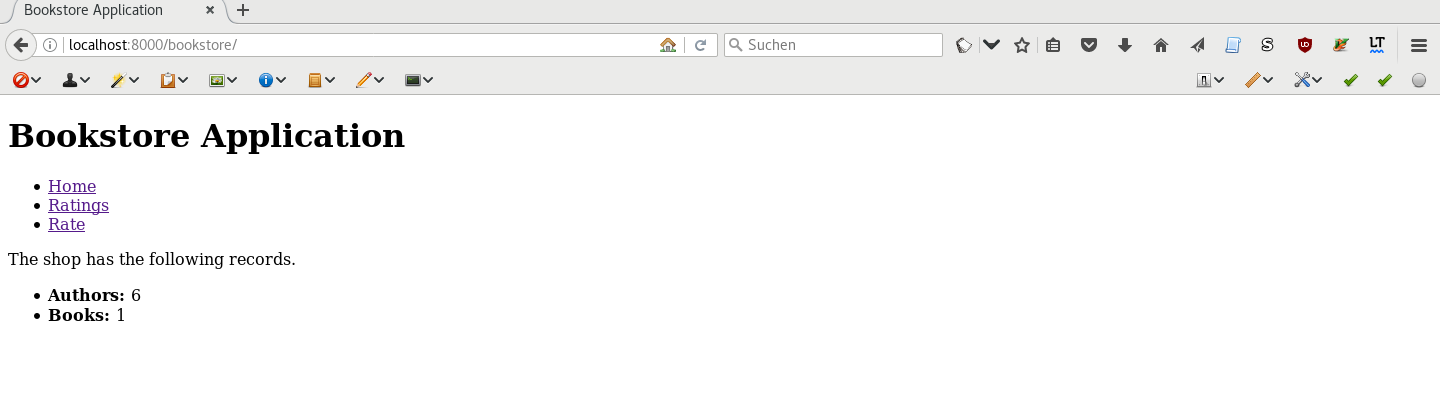
\includegraphics[scale=0.25]{images/Web-Application-Entry.png}
\caption{Web-Anwendung Startseite}
\label{fig:django-start}
\end{figure}

Derzeit gibt es zwei Benutzergruppen, welche verschiedene Bereiche der Anwendung
benutzen können. Die erste Gruppe ist die Gruppe der Administratoren, welche
Zugriff auf alle Funktionen der Anwendung haben. Die Administratoren können neue
Bücher anlegen, editieren oder löschen. Dies erfolgt über den von Django
bereitgestellte Administrator-Bereich. Der Administrator-Bereich ist eigentlich
die Admin-Anwendung. Eine Django-Anwendung ist eine spezielle Komponente, welche
genau eine Aufgabe erfüllt. Eine einmal entwickelte Anwendung sollte im
Ideal-Fall so konzipiert sein, dass sie in mehreren Django-Projekten zum Einsatz
kommen kann. In der Abbildung \ref{fig:django-create} ist die erzeugte Seite
für die Bücher dargestellt, welche vom der erwähnten Django-Admin Anwendung
erzeugt wurde.
Ein Django-Projekt besteht dabei zwingend aus mindestens einer
Django-Anwendung. Die Admin-Anwendung erzeugt dabei, für einmal definierte
Modelle, selbständig Oberflächen um die CRUD-Methoden bereitzustellen.

\begin{figure}
\centering
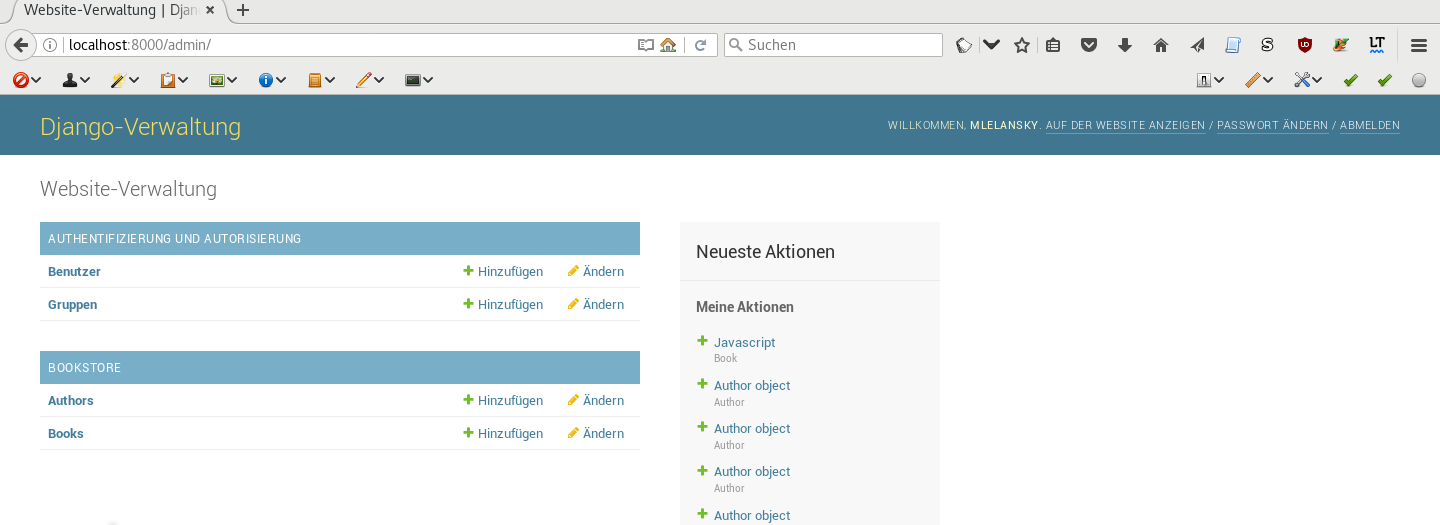
\includegraphics[scale=0.25]{images/Creation.png}
\caption{Büchererzeugung}
\label{fig:django-create}
\end{figure}

Die zweite Gruppe ist die Gruppe der normalen Benutzer, welche die eigentliche
Bewertung vornehmen können. Diese können aus einer Liste von registrierten
Büchern ein Buch auswählen und die dazugehörige Bewertung vornehmen. Die
Abbildung \ref{fig:django-rate} zeigt dabei die Formularseite, wo die Benutzer 
abstimmen können. Die Ergebnisseseite ist in der Abbildung \ref{fig:django-list}
dargestellt.

\begin{figure}
\centering
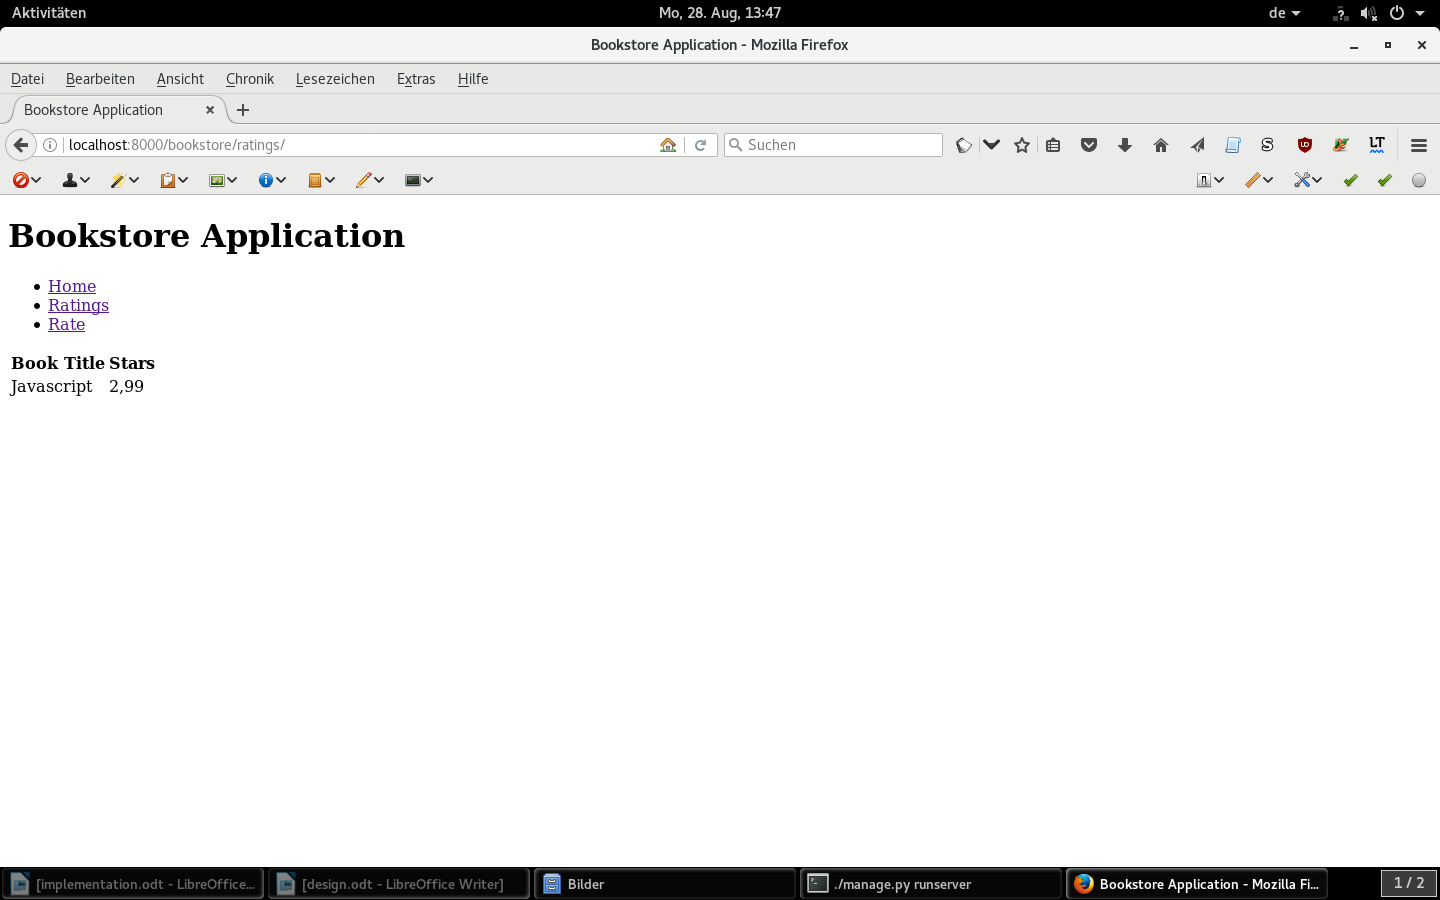
\includegraphics[scale=0.25]{images/Ratings.png}
\caption{Top-Liste}
\label{fig:django-list}
\end{figure}

\begin{figure}
\centering
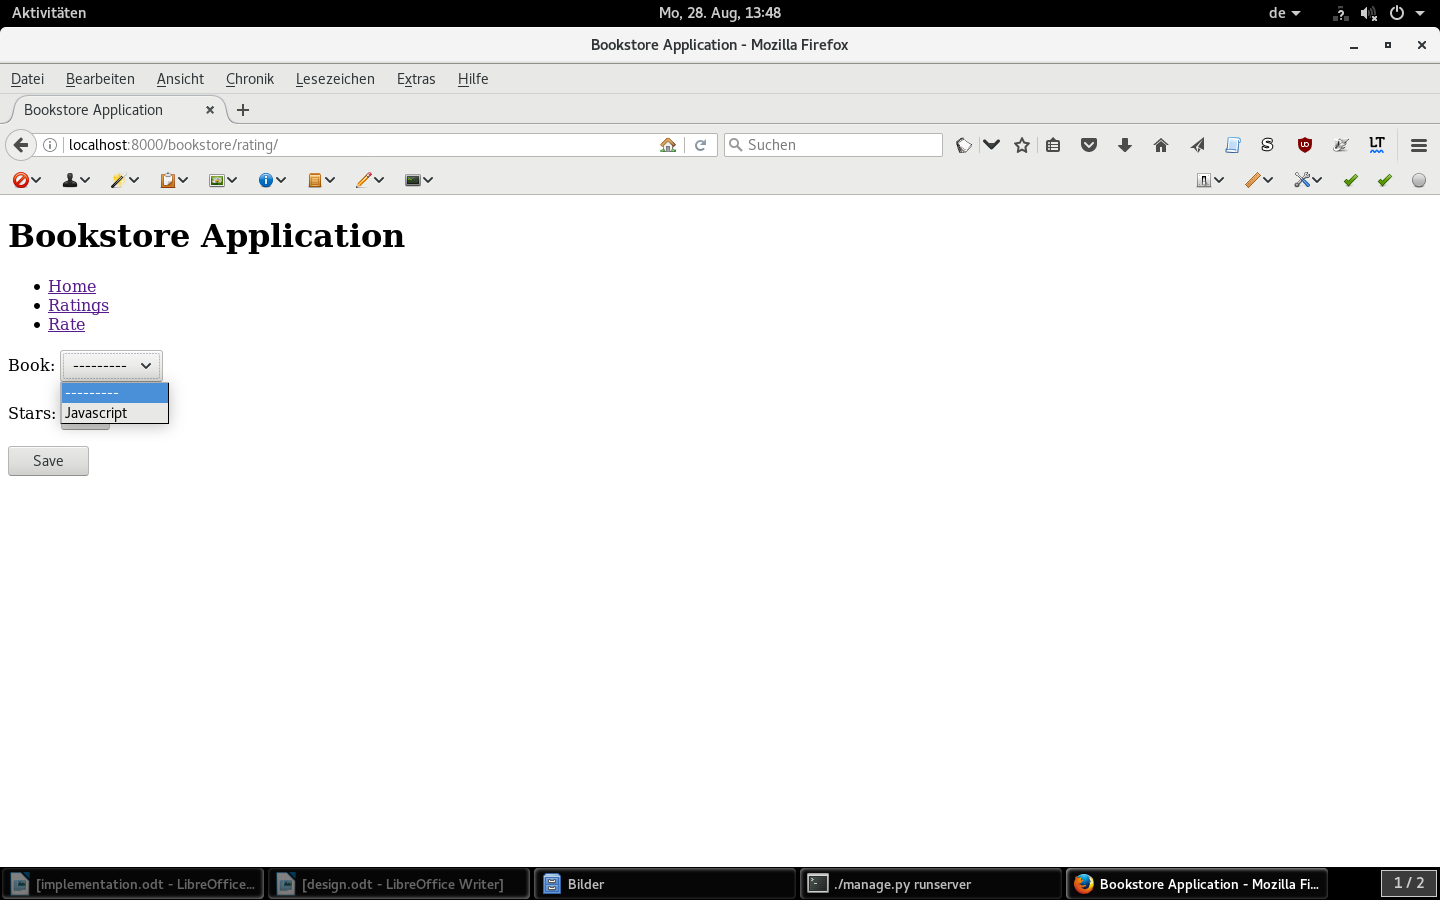
\includegraphics[scale=0.25]{images/Rating.png}
\caption{Rating von Büchern}
\label{fig:django-rate}
\end{figure}

Zusätzlich wurde noch ein Django-Kommando definiert um schnell viele Abstimmungen
vorzunehmen zu lassen.

\subsection{Anbindung der NoSql-Systeme}
Wie schon in der Design-Phase erwähnt, existiert für Memcached bereits eine
Django-Implementierung und auch die benötigten Client-Bibliotheken. Diese wurden
einfach in die bestehende Anwendung integriert, in dem die benötigten
Konfigurationseinstellungen vorgenommen wurden. Dabei wurde zusätzlich die Hilfe
der Bibliothek django-configurations\footnote{\url{https://pypi.python.org/pypi/django-configurations/2.0}}
benutzt um über einfache Optionsschalter die jeweiligen Cache"=Implementierungen
auszutauschen. Die Redis-Implementierung wurde nach dem gleichen Prinzip
übernommen.

Da der Voldemort-Client nicht funktionierte, wurde wie schon beschrieben ein
neuer \gls{REST}-Client entwickelt. Der Client wird dabei mit den Rest-Endpunkten
und den Node-Ids initialisiert. Danach kann der Anwender die Methoden frei
benutzen. Ein Abmelden, wie bei den anderen Bibliotheken ist hierbei nicht
notwendig, da alle Verbindungen über das HTTP-Protokoll laufen und nicht direkt
über Sockets. Danach wurde der neue Voldemort-Cache implementiert. Dabei wurde
die Django-Cache-Implementierung für Memcached als Ausgangsbasis genommen, da
von der API her Memcached und Voldemort ähnlich sind im Gegensatz zu Redis.

Bei der Anwendung sind alle Systeme gleich gut benutzbar. Je nach Anwendungsfall
kann man mehr oder weniger Aktionen von Django übernehmen lassen. Der einfachste
Fall ist Django die Speicherung der kompletten Anwendung zu überlassen. Etwas
mehr Kontrolle bekommt man, wenn man die Seiten, welche gespeichert werden
sollen selbst festlegt. Nochmals mehr Kontrolle erlangt man, wenn man nur Teile
einer Seite zwischenspeichert und die volle Kontrolle bekommt man, wenn man die
Zugriffsmethoden direkt verwendet. Diese Entscheidung muss jedoch jeder
Entwickler je nach Situation selber fällen.

\subsection{Probleme und offene Punkte bei der Umsetzung}
Trotz der erfolgreichen Anbindung von Voldemort an Django gibt es noch einige
Probleme, bzw. offene Punkte, welche man in einem weiteren
Implementierungsschritt umsetzen kann.

Das erste Problem ist die \gls{REST}-API von Voldemort, welche auch noch nicht
ganz ausgereift ist. Dies zeigt sich zum Beispiel im Verhalten mit den
Vektor-Uhren und Versionen. Außerdem kann es manchmal zu unkontrollierten
Verhalten beim  Speichern und Löschen kommen. Ein weiterer Punkt ist die Übergabe
der Serverinformationen, welche sich derzeit aus URL und Node-Id für den gesamten
Cluster zusammensetzt. Dies ist nicht wünschenswert, da normalerweise, der
Standard Java-Client und auch der rudimentäre Python-Client mit einem Server
des Clusters zufrieden sind und sich die restlichen Informationen vom Cluster
holen. Die normale REST-API bietet jedoch keine Möglichkeit die Metadaten des
Clusters abzufragen. Um die Metadaten des Clusters zu bekommen, muss erst der
existierende Koordinator-Service gestartet werden, welcher dann auch das
komplette Routing übernimmt.

Die Anwendung verfügt derzeit auch über keine Benutzerregistrierung, dies ist
aber notwendig um zu verhindern, dass jemand einen Artikel mehrfach bewertet.

Derzeit ist die entwickelte Anwendung nicht wie eine typische Django-Anwendung
wiederverwendbar, da die Domäne und das Abstimmungssystem in einer Anwendung sind.
Eine Verbesserung wäre es, wenn man das Abstimmungssystem unabhängig von den
einzelnen Produkten ist. Dazu müsste man die derzeitige Abhängigkeit in der
Tabelle zu den Produkten aufheben und die Information, für welches Produkt
abgestimmt wurde, redundant mit speichern.

\chapter{Zusammenfassung}
In diesem Kapitel geht es darum, die Ergebnisse nochmals zusammenzufassen und
einen Ausblick auf darauf aufbauende Möglichkeiten zu liefern.

\section{Fazit}
Die drei NoSql-Systeme wurden hinsichtlich ihrer Eigenschaften untersucht.
Dabei wurden die jeweiligen System kurz vorgestellt und ihre wichtigsten Punkte
erläutert. Danach wurden die ausgesuchten Eigenschaften verglichen. Dabei kam
heraus, dass Memcached und Redis sehr ähnlich konzipierte System sind. Dies ist
auch klar, da beide oft als Caches benutzt werden und Voldemort ist mehr wie
ein verteielter Speicher. Da alle Systeme die zu untersuchten Eigenschaften
unterschiedlich umgesetzt haben, ist es nicht möglich einen Favoriten zu
bestimmen. Welches System am besten geeignet ist, hängt vom geplanten
Einsatzzweck ab. Für Memcached wurde ein neues Performance-Tool entwickelt,
auch wenn nicht alle geplannten Funktionen umgesetzt wurden.

Der geplannte Anwendungsfall wurde trotzt der Schwierigkeiten von Voldemort
umgesetzt und je nach Bedarf können alle drei NoSql-Systeme benutzt werden.
Jedoch haben Memcached und Redis gegenüber Voldemort den Vorteil, dass sie schon
eine längere Entwicklungszeit hinter sich haben und deshalb sowohl die
NoSql-Systeme, wie auch Bibliotheken und Tools stabiler sind. Deshablb würde
ich nur Memcached und Redis im produktiven Einsatz empfehlen, da die Bibliothek
bei beiden Systemen ausgereifter sind, was einen Einsatz in unterschiedlichen
Systemen ermöglicht. Voldemort ist hier noch zu sehr auf die Java-Welt fixiert
und ist auch nur eingeschrängt verfügbar. Während Memcached, Redis und die
dazugehörigen Bibliotheken bei Linux über die Paketmanager verfügbar sind, bzw.
je nach Art der Programmiersprache auf den jeweiligen Seiten veröffentlicht sind,
ist dies bei Voldemort zum Zeitpunkt der Untersuchung nicht der Fall gewesen.
Es gibt jedoch schon Plannungen in die Richtung. Dies würde auch eine größere
Entwicklergemeinde erzeugen und den Unternehmen, die Möglichkeit geben über
mögliche Einsatzszenarien nachzudenken.

\section{Ausblick}
Für die zukünftigen Schritte ergeben sich zwei Möglichkeiten. Entweder man
entwickelt, das Benchmark-Tool für Memcached weiter oder man entwickelt ein
ähnliches Tool für Voldemort um dann zum Beispiel den gemeinsamen Nenner aller
drei Systeme zu vergleichen nämlich einen Text als Schlüssel und Wert zu
verwenden, welchen man in der Länge variable hällt. Dabei müsst das Tool für
Voldemort jedoch derzeit noch entweder in Java entwickelt werden oder über
entsprechende Bindings, wie \gls{JNI}, Jython, JRuby,~\dots{} verfügen.

Die andere Möglichkeit besteht, darin die Webseite weiter zu entwickeln und
dann darauf gewisse Lasttests zu fahren. Dadurch könnte man feststellen, welche
Systeme sich im Echtzeitbetrieb besser verhalten. Dazu müsste man jedoch dann
konsequent die Low-Level-Cache-API von Django benutzen, damit man auch die
Funktionalität von Redis benutzen kann um Listen und Mengen zu speichern.
Außerdem konnte man die in der Implementierung angesprochenen Probleme noch
umsetzen, wie die nichtvorhandene Benutzerregistrierung.

\printglossary
\listoffigures
\lstlistoflistings
\printbibliography
\end{document}
